\documentclass[10pt, a4paper]{article}
\usepackage[utf8]{inputenc}
\usepackage[spanish]{babel}
\usepackage[margin=1.5cm]{geometry}
\usepackage{graphicx}
\usepackage{booktabs}
\usepackage{hyperref}
\hypersetup{colorlinks=true, linkcolor=black, urlcolor=blue}
\usepackage{cleveref}
\usepackage{float}
\usepackage{etoolbox}
\usepackage{authblk}
\usepackage{xcolor}
\usepackage{caption}
\usepackage{subcaption}
\captionsetup{font=small}
\setlength{\parskip}{3pt}

\makeatletter
\apptocmd{\@floatboxreset}{\centering}{}{}
\makeatother

\title{\Large \textbf{Informe de rendimiento: Sistema de Reserva de Boletos}}
\author[1]{Solon Losada Cadena}
\author[1]{Juan Pablo Peña Bernal}
\author[1]{Alejandro González Ochoa}
\affil[1]{Departamento de Ingeniería de Sistemas, Pontificia Universidad Javeriana, Bogotá, Colombia.}
\date{22 de noviembre de 2026}

\begin{document}
\maketitle
\vspace{-1.2cm}
\begin{center}
	\small \textbf{Docente:} Ricardo Hjalmar González García
\end{center}

\section{Objetivo y alcance}
Este informe compara el desempeño de la arquitectura base del SRB (figura de tres capas del enunciado, un proceso de cada tipo) con la arquitectura escalable, que replica el servicio RMC, el servicio de cancelación y los hilos de persistencia. Se miden, con 3, 5 y 8 clientes simultáneos, el tiempo de respuesta (media y desviación estándar) y las transacciones por minuto (TPM) de las operaciones de consulta y de reserva.

\section{Entorno de medición}
\label{sec:entorno}
\textbf{Todos los procesos corrieron en una sola máquina}, no en las tres máquinas del despliegue; por eso las latencias de red no están incluidas y las cifras absolutas no son comparables con las de un despliegue distribuido. Lo que sí se compara es el efecto de replicar procesos bajo las mismas condiciones.

\begin{table}[H]
	\centering\small
	\begin{tabular}{@{}ll@{}}
		\toprule
		CPU & AMD Ryzen 7 5700U (8 núcleos, 16 hilos) \\
		RAM & 14 GiB \\
		Sistema operativo & Linux 7.3 (CachyOS) \\
		Lenguaje y librerías & Python 3.14, pyzmq 27.3 (ZeroMQ), SQLAlchemy 2.0, psycopg 3 \\
		Base de datos & PostgreSQL 16 en un contenedor Docker en la misma máquina \\
		Herramientas de medición & Generador de carga propio (\texttt{scripts/benchmark.py}), CSV por cliente y \texttt{statistics} de Python \\
		\bottomrule
	\end{tabular}
	\caption{Hardware y software de las mediciones.}
\end{table}

\section{Arquitecturas comparadas}
\begin{table}[H]
	\centering\small
	\begin{tabular}{@{}lcc@{}}
		\toprule
		Componente & Base & Escalable \\
		\midrule
		Gestor de transacciones (GT) & 1 & 1 \\
		Servicio RMC & 1 & 4 réplicas \\
		Servicio de cancelación y notificación & 1 & 2 réplicas \\
		Servicio de persistencia (hilos de atención) & 1 & 8 \\
		Supervisor (relanza procesos caídos) & sí & sí \\
		\bottomrule
	\end{tabular}
	\caption{Configuración de cada arquitectura. Las réplicas se conectan al GT, que reparte el trabajo con ROUTER/DEALER (RMC) y PUSH/PULL (cancelación).}
\end{table}

\section{Metodología}
\label{sec:metodo}
\textbf{Generación de carga.} Se usó un generador propio en Python (el diseño inicial mencionaba Locust; no se alcanzó a escribir su adaptador para ZeroMQ). Cada cliente es un \emph{proceso} independiente que envía solicitudes sincrónicas, una tras otra, durante 120 s. Los escenarios siguen el enunciado: con 3 clientes, 2 solo consultan y 1 consulta y reserva; con 5, 3 solo consultan y 2 reservan y modifican; con 8, 4 solo consultan y 4 reservan y modifican.

\textbf{Tasa.} El enunciado exige al menos 20 solicitudes por minuto por cliente. Con esa tasa ningún componente se acerca a su límite y ambas arquitecturas darían la misma respuesta, así que cada cliente se configuró a 6\,000 solicitudes por minuto, valor que ningún cliente alcanza: en la práctica cada uno envía la siguiente solicitud apenas recibe la respuesta (carga de ciclo cerrado) y el sistema trabaja a su máxima capacidad.

\textbf{Métricas.} El tiempo de respuesta es el medido por el cliente entre enviar la solicitud y recibir la respuesta; se reportan media y desviación estándar muestral por tipo de operación. Los TPM son las operaciones completadas (sin error técnico) divididas entre los minutos de la corrida, medidos en los clientes. Como contraste, el número de filas de la tabla de reservas en la BD coincide con las reservas exitosas. Antes de cada corrida la BD se recrea con 50 eventos (20 con dos ocurrencias) y \textbf{100\,000 asientos por ocurrencia}, en lugar de 100, para que el cupo no se agote durante los 120 s y distorsione la comparación.

\section{Resultados}
\label{sec:resultados}
\begin{table}[H]
	\centering\small
	\begin{tabular}{@{}rlrrrrr@{}}
\toprule
Clientes & Arquitectura & Consulta (ms) & Reserva (ms) & TPM consulta & TPM reserva & Errores \\
\midrule
3 & Base & 5.5 $\pm$ 3.1 & 8.5 $\pm$ 2.8 & 14\,488 & 2\,851 & 0 \\
3 & Escalable & 4.2 $\pm$ 1.1 & 8.7 $\pm$ 1.7 & 14\,810 & 2\,910 & 0 \\
\midrule
5 & Base & 17.4 $\pm$ 3.1 & 17.8 $\pm$ 3.0 & 10\,316 & 3\,459 & 0 \\
5 & Escalable & 5.5 $\pm$ 2.5 & 11.1 $\pm$ 3.0 & 17\,543 & 5\,287 & 0 \\
\midrule
8 & Base & 31.4 $\pm$ 4.5 & 31.7 $\pm$ 4.5 & 7\,636 & 3\,862 & 0 \\
8 & Escalable & 13.5 $\pm$ 7.8 & 20.7 $\pm$ 7.1 & 16\,026 & 6\,053 & 0 \\
\bottomrule
\end{tabular}

	\caption{Resultados por escenario: tiempo medio $\pm$ desviación estándar (ms), TPM de cada operación y errores técnicos (timeouts).}
	\label{tab:resultados}
\end{table}

\begin{figure}[H]
	\centering
	\begin{subfigure}{0.49\textwidth}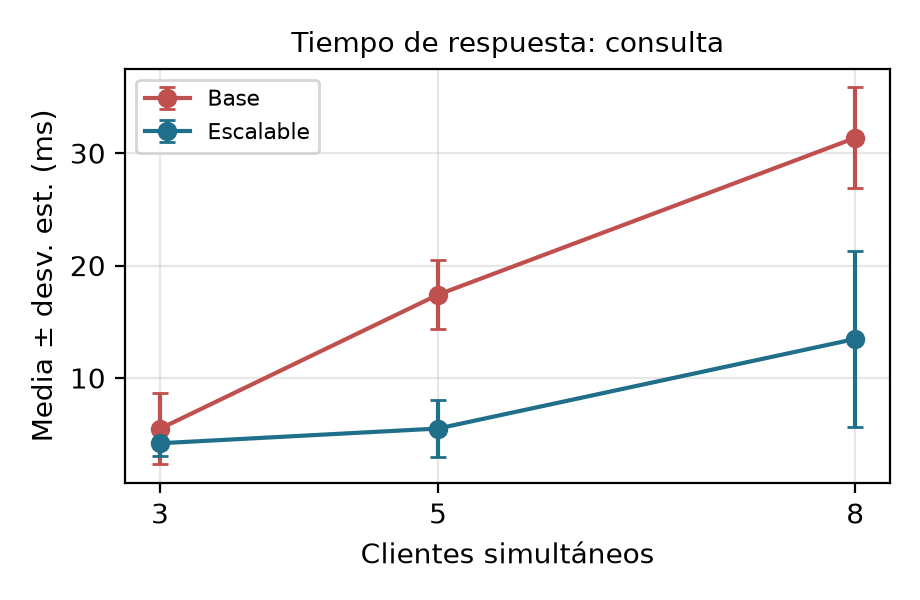
\includegraphics[width=\textwidth]{Images/rend_consulta_ms.png}\end{subfigure}
	\begin{subfigure}{0.49\textwidth}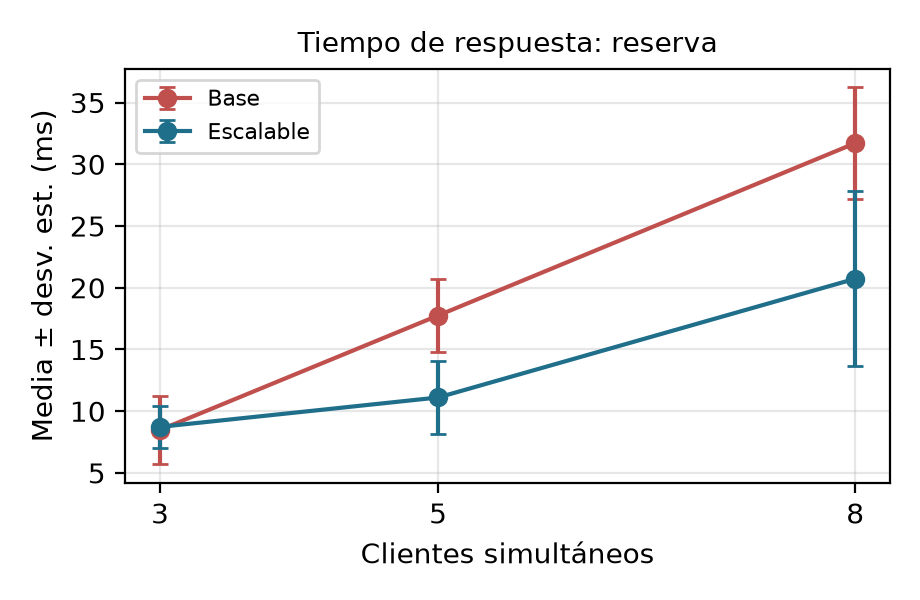
\includegraphics[width=\textwidth]{Images/rend_reserva_ms.png}\end{subfigure}
	\begin{subfigure}{0.49\textwidth}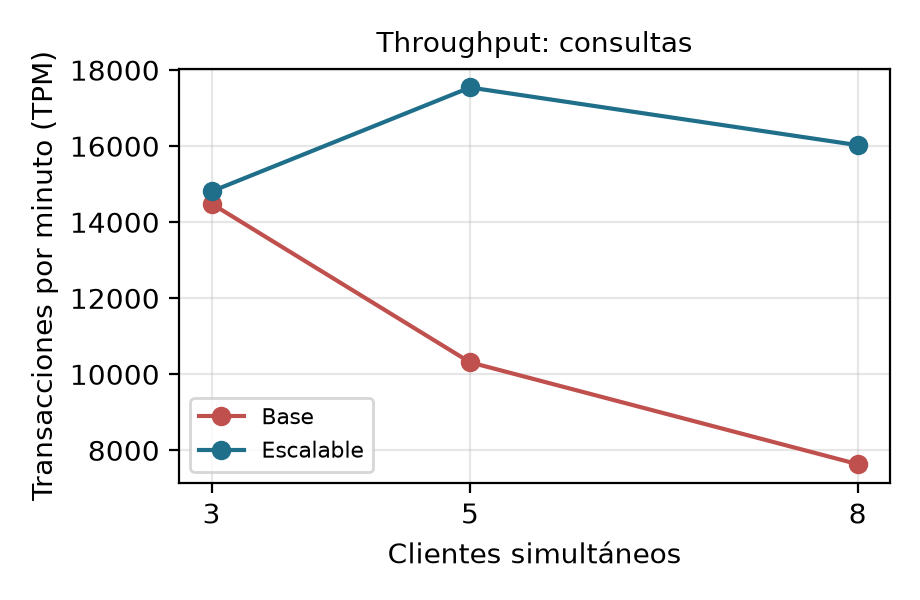
\includegraphics[width=\textwidth]{Images/rend_consulta_tpm.png}\end{subfigure}
	\begin{subfigure}{0.49\textwidth}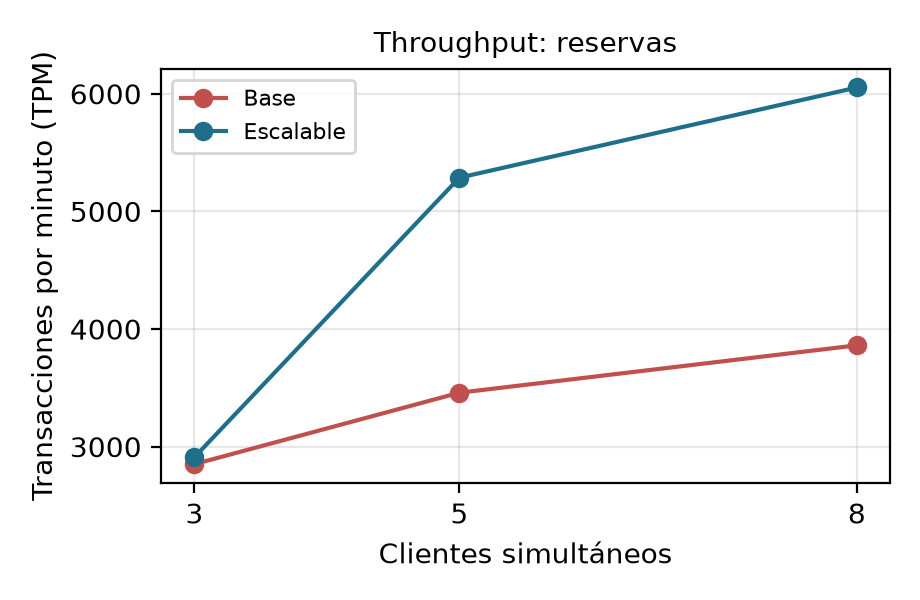
\includegraphics[width=\textwidth]{Images/rend_reserva_tpm.png}\end{subfigure}
	\caption{Tiempo de respuesta (arriba, media con barras de desviación estándar) y transacciones por minuto (abajo) frente al número de clientes, para la arquitectura base y la escalable.}
	\label{fig:graficas}
\end{figure}

\section{Análisis}
\label{sec:analisis}
\textbf{Con 3 clientes no hay diferencia.} Solo un cliente reserva, y un RMC con un hilo de persistencia lo atiende sin cola: la reserva tarda 8.5 ms en la arquitectura base y 8.7 ms en la escalable, y los TPM difieren en 2\,\%, dentro del ruido (la desviación estándar es de 2 a 3 ms). La consulta pasa de 5.5 a 4.2 ms, pero con desviaciones de 3.1 y 1.1 ms no hay base para atribuirlo a la arquitectura. Replicar no cuesta rendimiento cuando la carga es baja.

\textbf{Con 5 y 8 clientes la arquitectura base se satura.} Su tiempo de respuesta sube casi en proporción al número de clientes: la consulta pasa de 5.5 ms (3 clientes) a 17.4 (5) y 31.4 ms (8), y la reserva de 8.5 a 17.8 y 31.7 ms. Los TPM no crecen: los de consulta bajan de 14\,488 a 7\,636 al pasar de 3 a 8 clientes, aunque haya más clientes pidiendo. Este comportamiento es el de un sistema con capacidad fija (un RMC, un hilo de persistencia) al que llegan más solicitudes de las que procesa: las solicitudes esperan en cola y la latencia crece. No medimos en qué componente se forma la cola; la hipótesis más probable es el RMC y el hilo único de persistencia, que son lo que cambia entre arquitecturas.

\textbf{La arquitectura escalable absorbe la carga adicional.} Con 5 clientes baja el tiempo de consulta 68\,\% (17.4 a 5.5 ms) y el de reserva 37\,\% (17.8 a 11.1 ms), y los TPM suben 70\,\% y 53\,\%. Con 8 clientes la consulta baja 57\,\% (31.4 a 13.5 ms) y la reserva 35\,\% (31.7 a 20.7 ms); los TPM de consulta se multiplican por 2.1 (7\,636 a 16\,026) y los de reserva por 1.6 (3\,862 a 6\,053). No hubo errores técnicos en ninguna de las seis corridas.

\textbf{Por qué la mejora es menor que el número de réplicas.} Con 4 réplicas de RMC no se obtiene 4 veces más rendimiento. Las reservas mejoran menos que las consultas. Son hipótesis, no mediciones: (i) el GT sigue siendo un único proceso por el que pasan todas las solicitudes; (ii) una reserva hace dos consultas a persistencia y una transacción de escritura sobre una sola base PostgreSQL, que serializa las escrituras sobre la misma fila; (iii) los clientes, los servicios y la base compartieron los mismos núcleos de una sola máquina. Con 8 clientes la desviación de la arquitectura escalable (7.8 ms en consulta) es mayor que la de la base (4.5 ms), lo que es coherente con ese reparto desigual de CPU, aunque no lo comprobamos.

\textbf{Efecto de la réplica de PostgreSQL.} Con la arquitectura escalable y 8 clientes se repitió la medición con la réplica en streaming activa: las consultas de eventos se leyeron de la réplica (más de 32\,000 lecturas contabilizadas en ella; primario y réplica terminaron con las mismas 12\,146 reservas y un retraso de replicación de 1.4 ms). Los resultados son equivalentes a los de la corrida sin réplica: consulta 13.4 $\pm$ 7.8 ms y 16\,045 TPM (antes 13.5 $\pm$ 7.8 ms y 16\,026 TPM), reserva 20.8 $\pm$ 7.1 ms y 6\,061 TPM (antes 20.7 $\pm$ 7.1 ms y 6\,053 TPM), sin errores. Es esperable: las tablas son pequeñas, una lectura tarda alrededor de un milisegundo de los 13 ms de una consulta, y la base y la réplica comparten los mismos núcleos. Lo que aporta la réplica en este sistema es una copia de los datos y la capacidad de seguir atendiendo consultas si cae el nodo primario o la propia réplica, no más velocidad.

\textbf{Atributos de calidad y patrones.} \emph{Escalabilidad:} el patrón ROUTER/DEALER entre GT y RMC, y PUSH/PULL hacia cancelación, permitió añadir réplicas sin modificar el GT ni los clientes, porque las réplicas se conectan al GT y este reparte por turnos. \emph{Desempeño:} la mejora aparece solo cuando hay saturación; a 20 solicitudes por minuto por cliente (el mínimo del enunciado) ambas arquitecturas darían tiempos equivalentes. \emph{Tolerancia a fallos:} en una prueba aparte (\texttt{scripts/demo\_fallos.py}) se enviaron 24 reservas seguidas matando con \texttt{kill -9} el GT (dos veces) y un RMC; el supervisor relanzó cada proceso y el cliente reintentó con el mismo identificador. Las 24 reservas quedaron guardadas una sola vez en la base (0 duplicadas). Las operaciones afectadas tardaron unos 2.5 s (el tiempo de espera del cliente antes de reintentar) frente a unos 20 ms habituales; ese es el costo de la recuperación transparente.

\textbf{Respuesta a la pregunta del enunciado.} En este experimento el diseño escalable mejora las métricas solo cuando el sistema está saturado: con 5 y 8 clientes reduce el tiempo de consulta entre 57\,\% y 68\,\% y el de reserva entre 35\,\% y 37\,\%, y aumenta el throughput de consulta entre 70\,\% y 110\,\% y el de reserva entre 53\,\% y 57\,\%. Con 3 clientes no hay mejora apreciable.

\section{Limitaciones}
\begin{itemize}
	\item Todo corrió en una máquina, con el cliente, los servicios y PostgreSQL compitiendo por la misma CPU. En el despliegue de tres máquinas la red añade latencia y las capas no compiten por recursos.
	\item La réplica de PostgreSQL se añadió después de las seis corridas principales, que se hicieron con una sola base; solo se midió una corrida adicional con ella (arquitectura escalable, 8 clientes, ver arriba). Su efecto sobre el rendimiento en una sola máquina es nulo, y no se midió su efecto con la base y la réplica en máquinas distintas.
	\item Cada configuración se midió una vez (120 s); no se calcularon intervalos de confianza entre repeticiones.
	\item La tasa de 6\,000 solicitudes por minuto por cliente (ciclo cerrado) supera el mínimo del enunciado a propósito, para observar la saturación.
\end{itemize}

\end{document}
